



%%%%%
\section{The Tangent Bundle of Vector Bundles}

\TOX{
This section follows \cite{kolar1999natural} and \cite{michor2008topics} closely.

See also %\cite{szilasi2013connections}
}

Let $(E,\pi,M)$ be a vector bundle, and denote 
$$+_E:E\times_ME\to E,\qquad +_E((x,u),(x,v))=(x,u+v),$$
fiberwise addition and
$$m_t^E:E\to E,\qquad m_t^E(x,v)=(x,tv),$$
fiberwise scalar multiplication.

As usual, since $E$ is a smooth manifold, we have the tangent bundle $(TE,\pi_E,E)$ which is again a smooth vector bundle with fiberwise addition $+_TE$ and fiberwise scalar multiplication $m_t^{TE}$.  We wish to see how the bundle charts of $(TE,\pi_E,E)$ relate to the bundle charts of $(E,\pi,M)$.

Suppose $(E,\pi,M)$ is a vector bundle with bundle atlas $\{(U_\alpha,\psi_\alpha):\psi_\alpha:\rest{E}_{U_\alpha}\to U_\alpha\times V\}$ such that $\{(U_\alpha,\phi_\alpha):\phi_\alpha:U_\alpha\to\phi_\alpha(U_\alpha)\subseteq\R^n\}$ is a smooth atlas for $M$.  Then $\{(\rest{E}_{U_\alpha},\tilde{\phi}_\alpha):\tilde{\phi}_\alpha:\rest{E}_{U_\alpha}\to\phi_\alpha(U_\alpha)\times V\}$ is a compatible smooth atlas for $E$, where
$$\tilde{\phi}_\alpha=(\phi_\alpha\times\id_V)\circ\psi_\alpha:\rest{E}_{U_\alpha}\to\phi_\alpha(U_\alpha)\times V.$$
Then our atlas for $TE$ is given by $\{(T(\rest{E}_{U_\alpha}),d\tilde{\phi}_\alpha)\}$
where
$$d\tilde{\phi}_\alpha:T(\rest{E}_{U_\alpha})\to T(\phi_\alpha(U_\alpha)\times V)=(\phi_\alpha(U_\alpha)\times V)\times(\R^n\times V).$$


For $p\in U_{\alpha\beta}$ and $x=\phi_\beta(p)$, and $v,w\in V$, $\xi\in\R^n$ we have the transition functions
$$\phi_\alpha\circ\phi_\beta^{-1}(x)=\phi_{\alpha\beta}(x),$$
$$\psi_\alpha\circ\psi_\beta^{-1}(p,v)=(p,\psi_{\alpha\beta}(p)v),$$
\begin{align*}
	\tilde{\phi}_\alpha\circ\tilde{\phi}_\beta^{-1}(x,v)&=(\phi_\alpha\times\id_V)\circ\psi_\alpha\circ\psi_\beta^{-1}\circ(\phi_\beta^{-1}\times\id_V)(x,v)\\
	&=(\phi_\alpha\times\id_V)\circ\psi_\alpha\circ\psi_\beta^{-1}(p,v)\\
	&=(\phi_\alpha\times\id_V)(p,\psi_{\alpha\beta}(p)v)\\
	&=(\phi_{\alpha\beta}(x),\psi_{\alpha\beta}(\phi_\beta^{-1}(x))v),
\end{align*}
and
\begin{align*}
	d\tilde{\phi}_\alpha\circ & d\tilde{\phi}_\beta^{-1}(x,v;\xi,w)=d(\tilde{\phi}_\alpha\circ\tilde{\phi}_\beta^{-1})_{(x,v)}(\xi,w)\\
	&=(\phi_{\alpha\beta}(x),\psi_{\alpha\beta}(\phi_\beta^{-1}(x))v;d(\phi_{\alpha\beta})_x(\xi),d(\psi_{\alpha\beta}\circ\phi_\beta^{-1})_x(\xi)v+\psi_{\alpha\beta}(\phi^{-1}(x))w).
\end{align*}
That is, letting $\tilde{\psi}_\alpha=d\tilde{\phi}_\alpha$, we have the transition maps 
$$\tilde{\psi}_{\alpha\beta}:\rest{E}_{U_{\alpha\beta}}\to GL(\R^n\times V),$$
$$(p,v)\mapsto \begin{pmatrix}(d(\phi_\alpha)_p&0\\
 	v\cdot d(\psi_{\alpha\beta})_p&\psi_{\alpha\beta}(p)
 \end{pmatrix},$$
 where we have identifies $d(\phi_\beta)_p:T_pM\congto\R^n$.  Thus we have described the vector bundle structure of $(TE,\pi_E,E)$ in terms of our other structures.
 
 Note from the above, when considering $(p,\xi)\in TU_{\alpha\beta}$, then we have a similar map
 $$TU_{\alpha\beta}\to GL(V\times V),\qquad (p,\xi)\mapsto \begin{pmatrix}\psi_{\alpha\beta}(p)&0\\
 	\xi\cdot d(\psi_{\alpha\beta})_p&\psi_{\alpha\beta}(p)
 \end{pmatrix}.$$
 This shows that $(TE,d\pi,TM)$ is a vector bundle as well with fiberwise addition $d(+_E)$ and fiberwise scalar multiplication $d(m_t^E)$.
 
 Thus when $(E,\pi,M)$ has an appropriately chosen vector bundle structure, we obtain the natural tangent bundle $(TE,\pi_E,E)$ structure in correlation with the former structure, and we obtain another vector bundle structure $(TE,d\pi, TM)$ which can be considered as the differential of the original one.
 
 Recall that an \textit{exact sequence} is a sequence of the form
 \begin{center}
	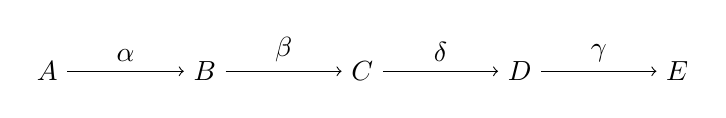
\begin{tikzpicture}[auto, node distance=2cm]
		\node(A){$A$};
		\node(B)[right of=A]{$B$};
		\node(C)[right of=B]{$C$};
		\node(D)[right of=C]{$D$};
		\node(E)[right of=D]{$E$};
		\draw[->](A) to node{$\alpha$}(B);
		\draw[->](B) to node{$\beta$}(C);
		\draw[->](C) to node{$\delta$}(D);
		\draw[->](D) to node{$\gamma$}(E);
	\end{tikzpicture}
\end{center}
where
$$\im{\alpha}=\ker{\beta},\qquad \im{\beta}=\ker{\delta},\qquad \im{\delta}=\ker{\gamma}.$$
And a \textit{short exact sequence} is an exact sequence of the form
 \begin{center}
	\begin{tikzpicture}[auto, node distance=2cm]
		\node(A){$0$};
		\node(B)[right of=A]{$A$};
		\node(C)[right of=B]{$B$};
		\node(D)[right of=C]{$C$};
		\node(E)[right of=D]{$0$};
		\draw[->](A) to node{}(B);
		\draw[->](B) to node{$\alpha$}(C);
		\draw[->](C) to node{$\beta$}(D);
		\draw[->](D) to node{}(E);
	\end{tikzpicture}
\end{center}

\begin{prop}
    Let $(E,\pi, M)$ be a smooth vector bundle.  There exists a canonical short exact sequence
     \begin{center}
	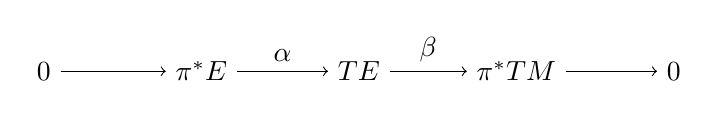
\begin{tikzpicture}[auto, node distance=2cm]
		\node(A){$0$};
		\node(B)[right of=A]{$\pi^*E$};
		\node(C)[right of=B]{$TE$};
		\node(D)[right of=C]{$\pi^*TM$};
		\node(E)[right of=D]{$0$};
		\draw[->](A) to node{}(B);
		\draw[->](B) to node{$\alpha$}(C);
		\draw[->](C) to node{$\beta$}(D);
		\draw[->](D) to node{}(E);
	\end{tikzpicture}
\end{center}
of vector bundles.
\end{prop}

\begin{proof}
Let's first unravel notation:  

Recall that
$$\pi^*E=\{(u,v)\in E\times E:\pi(u)=\pi(v)\}\cong E\oplus E,$$
and as a bundle $\pi_1:E\oplus E\to E$ with projection onto the first factor.  Post composing with $\pi$, we obtain a vector bundle $E\oplus E\to M$.

We have $(TE,\pi_E,E)$ as the usual tangent bundle of $E$, and post composing with $\pi$ we obtain a vector bundle $TE\to M$.

Let $\iota:TM\to TE$ be the zero section, and let $\pi^*TM=\iota(TM)$ denote the the subbundle of $d\pi:TE\to TM$ and then post composing with $\pi_M:TM\to M$ yields the vector bundle $\pi^*TM\to M$.

Define the map $\alpha:\pi^*E\to TE$ by
$$\alpha(u,v)=\left(p,u;0,\rest{\frac{d}{dt}}_{t=0}(u+tv)\right).$$

Define the map $\beta:TE\to \pi^*TM$ by
$$\beta(x,v;\xi,w)=(x,0;\xi,0),$$
i.e., $\beta=\iota\circ d\pi$.  Then we see that
\begin{align*}
	\beta\circ\alpha((x,v),(x,w))&=\beta\left(x,v;0,\rest{\frac{d}{dt}}_{t=0}(v+tw)\right)\\
	&=(x,0;0,0).
\end{align*}
Hence $\im{\alpha}\subseteq\ker{\beta}.$  Moreover, since $\pi^*TM$ is a rank $n$ vector bundle over $M$ and $TE$ is a rank $n+2k$ vector bundle over $M$, we have that $\ker{\beta}$ is $2k$-dimensional, as is $\im{\alpha}$ by construction.  Thus by dimensionality, we have that $\im{\alpha}=\ker{\beta}$.  Moreover, by construction $\alpha$ is injective and $\beta$ is surjective thus showing exactness.
\end{proof}


 
 
 
 
 %%%%%
 \subsection{The Vertical Bundle}
 
Let $\pi:E\to M$ and consider the associated bundle $d\pi:TE\to TM$.  Thinking of $d\pi$ as a bundle homomorphism, we have the following commutative diagram
\begin{center}
	\begin{tikzpicture}[auto, node distance=3cm]
		\node(A){$TE$};
		\node(B)[right of=A]{$TM$};
		\node(C)[below of=A]{$E$};
		\node(D)[right of=C]{$M$};
		\draw[->](A) to node{$d\pi$}(B);
		\draw[->](A) to node[swap]{$\pi_E$}(C);
		\draw[->](B) to node{$\pi_M$}(D);
		\draw[->](C) to node[swap]{$\pi$}(D);
	\end{tikzpicture}
\end{center}
In local coordinates, we have that $d\pi(x,v;\xi,w)=(x,\xi)$.  That is, for each $(x,v)\in E$, the map $d\pi_{(x,v)}:T_{(x,v)}E\to T_xM$ has constant rank $n$.  Thus $\ker{d\pi}$ is a vector subbundle of $(TE,\pi_E,E)$ where
$$(\ker{d\pi})_\theta=\ker{d\phi_\theta}.$$
Moreover, since $TE$ is a rank $n+k$ vector bundle over $E$, we have that $\ker{d\pi}$ is a rank $k$ vector subbundle by dimensionality.

We define the \textit{vertical bundle over $E$} to be
$$VE:=\ker{d\pi}.$$
The local form of a vertical vector $X\in VE$ is given by
$$X=(x,v;0,w).$$
Moreover, since the transition functions
$$d\tilde{\phi}_\alpha\circ d\tilde{\phi}_\beta^{-1}(x,v;0,w)=(\phi_{\alpha\beta}(x),\psi_{\alpha\beta}(\phi_\beta^{-1}(x))v;0,\psi_{\alpha\beta}(\phi_\beta^{-1}(x))w)$$
are linear in $(v,w)\in V\times V$ for fixed $x$, we see that $VE$ is actually a vector bundle over $M$ of rank $2k$.

Let $\iota:M\to TM$ denote the zero section of $(TM,\pi_M,M)$.  Then consider the pullback bundle $\iota^*(TE,d\pi,TM)$
\begin{center}
	\begin{tikzpicture}[auto, node distance=3cm]
		\node(A){$\iota^*TE$};
		\node(B)[right of=A]{$TE$};
		\node(C)[below of=A]{$M$};
		\node(D)[right of=C]{$TM$};
		\draw[->](A) to node{$\iota_\#$}(B);
		\draw[->](A) to node[swap]{$\iota^*d\pi$}(C);
		\draw[->](B) to node{$d\pi$}(D);
		\draw[->](C) to node[swap]{$\iota$}(D);
	\end{tikzpicture}
\end{center}
and recall that
\begin{align*}
	\iota^*TE&=\{(x,(y,v;\xi,w))\in M\times TE:\iota(x)=d\pi(y,v;\xi,w)\}\\
	&=\{(x,(y,v;\xi,w))\in M\times TE:x=y\text{ and } \xi=0\}\\
	&\cong VE.
\end{align*}
Thus we may think of the vertical bundle as the pullback via the zero section.  Moreover, we have a canonical isomorphism $\vl:E\oplus E\to VE$ given by
$$\vl(u_p,v_p)=\rest{\frac{d}{dt}}_{t=0}(u_p+tv_p).$$
In local coordinates
$$\vl((x,u),(x,v))=(x,u;0,v).$$
The map $\vl$ is called the \textit{vertical lift}.  We define the \textit{vertical projection} to be the map $\vpr:VE\to E$ given by
$$\vpr:=\pi_2\circ\vl^{-1},$$
where $\pi_2:E\oplus E\to E$, $\pi_2(u,v)=v.$  Note that
$$\pi_1\circ\vl^{-1}=\rest{\pi_E}_{VE}.$$





%%%%%
\subsection{The Double Tangent Bundle}

Consider the tangent bundle $\pi:TM\to M$ as a vector bundle in its own right.  Then from preceding remarks, we have two canonical vector bundle structures on the double tangent bundle $TTM\to TM$.  The first is as the tangent bundle to the tangent bundle given by $\pi_{TM}:TTM\to TM$.  The second is as the differential $d\pi:TTM\to TM$.

We wish to see how $(TTM, d\pi, TM)$ and $(TTM, \pi_{TM}, TM)$ are related.  To this end, define the \textit{canonical flip} $\kappa:TTM\to TTM$ given in local coordinates by
$$\kappa(x,v;\xi,\eta)=(x,\xi;v,\eta).$$
Then
$$d\pi\circ\kappa=\pi_{TM}$$
and
$$\pi_{TM}\circ\kappa=d\pi.$$
Moreover, it's clear that $\kappa^{-1}=\kappa$.

\begin{prop}
    $\kappa:TTM\to TTM$ is the unique smooth mapping such that
    $$\pfrac{}{s}\pfrac{}{t}\Gamma(s,t)=\kappa(\pfrac{}{t}\pfrac{}{s}\Gamma(s,t))$$
    for any smooth $\Gamma:\R^2\to M$.
\end{prop}

Recall that for a vector field $X\in\vf{M}$, we may treat $X$ as smooth map $X:M\to TM$, and hence we have the differential $dX:TM\to TTM$.

\begin{prop}
    For $X,Y\in\vf{M}$, we have that
    $$[X,Y]=\vpr\circ(dY\circ X-\kappa\circ dX\circ Y)$$
    and
    $$dY\circ X-\kappa\circ dX\circ Y=\vl(Y,[X,Y]).$$
\end{prop}

\begin{proof}
Recall that in local coordinates, we have that
\begin{align*}
	[X,Y]&=X[Y^j]\partial_j-Y[X^j]\partial_j\\
	&=X^i\pfrac{Y^j}{x^i}\partial_j-Y^i\pfrac{X^j}{x^i}\partial_j\\
	&=dY^j(X)\partial_j-dX^j(Y)\partial_j.
\end{align*}
Now, treating $X,Y:M\to TM$ as a smooth map, we have in local coordinates that
$$X(x)=(x,\cl{X}(x)),\qquad Y(x)=(x,\cl{Y}(x)).$$
Then as a map $dX_p:T_pM\to T_{X(p)}TM$ we have the local expression
$$dX_p=
\begin{pmatrix}
\id_{T_pM}\\
d\cl{X}_p
\end{pmatrix},$$
and hence for $Y\in TM$, we see that that
$$dX\circ Y(x)=(x,\cl{X}(x);\cl{Y}(x),d\cl{X}_x(\cl{Y}_x)).$$
It's clear from this that the first expression follows, as does the second from our local expression of vertical lift.
\end{proof}



 
 
















